%=============================================================================
\documentclass[10pt,a4paper]{article}
%
%
%
%
\usepackage{graphicx}
\usepackage{hyperref}
\usepackage{verbatim}
\usepackage{fix-cm}
\usepackage{lineno}
\usepackage{fancyhdr}
%\usepackage{amsmath}
%
\oddsidemargin  0.1 in
\evensidemargin 0.1 in
%
%
\newlength{\backindent}\setlength{\backindent}{2cm}
\textwidth 5.375 in % Width of text line.
\advance\textheight by1.4cm
\advance\voffset by-1.4cm
\advance\textwidth by\backindent
%
%
% === Fancy headers setup  ===============================
%
\setlength{\headheight}{15.2pt}
\pagestyle{fancyplain} {
\fancyhead[L]{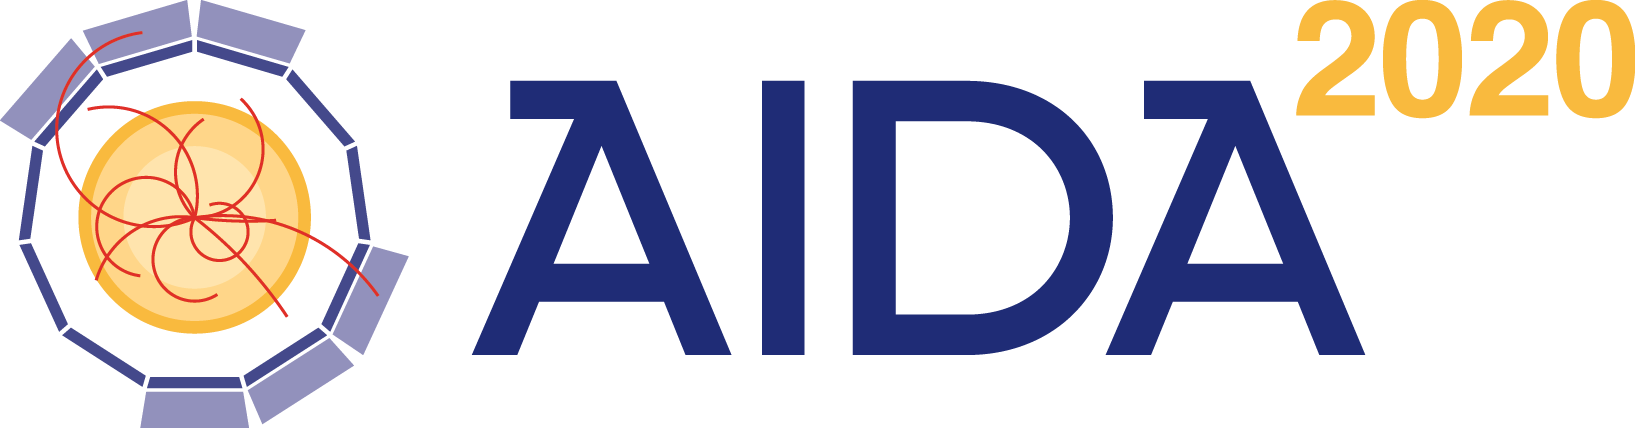
\includegraphics[height=10mm]{./setup/AIDA2020-logo}\vspace{-0.3cm}}
\fancyhead[C]{}
\fancyhead[R]{\sffamily{\underline{\hspace{6cm}Advanced European Infrastructures for Detectors at Accelerators}}}
\fancyfoot[L]{}
\fancyfoot[C]{\sffamily{User Manual}}
\fancyfoot[R]{\sffamily{\thepage}}
}
%
%
\newcommand{\tw}[1]{${\tt{#1}}$}
\newcommand{\tts}[1]{{\tt\small{#1}}}
\newcommand{\bold}[1]{{\bf{#1}}}
%
%
\newcommand{\docline}[2]{\vspace{0.1cm}{\bf{#1}} & \parbox{14.5cm}{#2}\\}
%
% === Specialization of the lineno package
%
\renewcommand{\linenumberfont} {\normalfont\small\sffamily}
\renewcommand{\makeLineNumber} {\makeLineNumberLeft}
\renewcommand{\linenumbersep} {2pt}
%
% === Set font to code section with line numbers
%
\newenvironment{code}{\par\vspace{0.01cm}\small\linenumbers\verbatim\setcounter{linenumber}{1}}{\endverbatim\nolinenumbers\vspace{-0.02cm}}%
%
% === Set font to code section with line numbers
%
\newenvironment{unnumberedcode}{\par\vspace{-0.1cm}\small\verbatim\setcounter{linenumber}{1}}%
{\endverbatim\vspace{-0.2cm}}
%
%
% ===  Compactify the item list  =========================
%
\newcommand{\itemcompact}{\setlength{\itemsep}{1pt}\setlength{\parskip}{0pt}\setlength{\parsep}{0pt}}
%
%
% ===  Title page command  ===============================
%
%
\newcommand{\basictitle}[2]{
%
\pagestyle{empty}
%
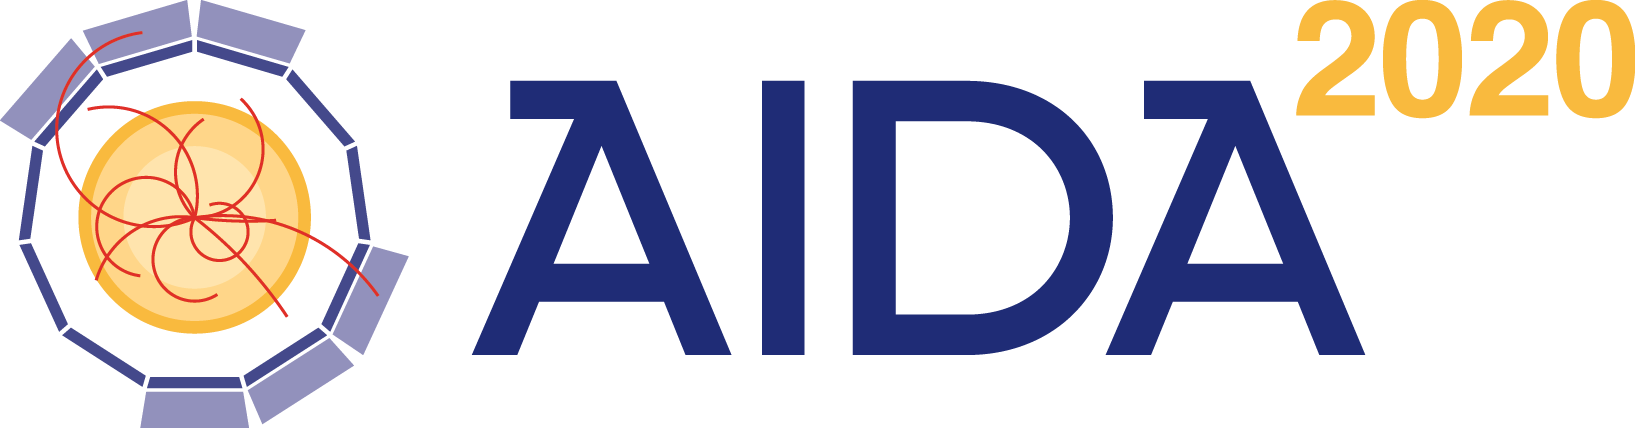
\includegraphics[height=25mm] {./setup/AIDA2020-logo}

\vspace{0.02cm}

{\sffamily{\underline{\hspace{6cm}Advanced European Infrastructures for Detectors at Accelerators}}}

\vspace{2cm}

\begin{center}
{\fontsize{72}{32}\selectfont{\bfseries{#1}}}

\vspace{3cm}
{\Huge\bf{#2}}
\vspace{3cm}
\begin{figure}[b]
  \begin{center}
    
\includegraphics[height=15mm] {./setup/Horizon2020-grant-logo}
  \end{center}
\end{figure}
\end{center}
}
\newcommand{\AIDAtitle}[3]{
\begin{titlepage}
\basictitle{#1}{#2}
\begin{center}
{#3}
\end{center}
\end{titlepage}
}

%
% === Command to insert http links to the DD4hep geomtery package
%
\newcommand{\detdesc}[2]
{
    \href{http://www.cern.ch/frankm/DD4hep/#1}{#2}
}
%
% === Command to insert http links to the ROOT geomtery package
%
\newcommand{\tgeo}[2]
{
    \href{http://root.cern.ch/root/html/#1.html}{#2}
}
\newcommand{\tgeoO}[3]
{
    \href{http://root.cern.ch/root/html/#1:#2}{#3}
}
\newcommand{\DDE}{{$\tt{DDEve}$\space}}
\newcommand{\DDhep}{{$\tt{DD4hep}$\space}}
\newcommand{\DDH}{{$\tt{DD4hep}$\space}}
\newcommand{\DDG}{{\tt{DDG4}\space}}
\newcommand{\DDA}{{\tt{DDAlign}\space}}
\newcommand{\DDC}{{\tt{DDCond}\space}}
\newcommand{\DDR}{{\tt{DDRec}\space}}
%
% ===  Custom title page  ================================
%
\newcommand{\mytitle}[3]{
\begin{titlepage}
\basictitle{#1}{#2}
\begin{center}
{#3}
\end{center}
\end{titlepage}
}

%
\pagestyle{fancyplain}{\fancyfoot[C]{\sffamily{DDG4 User Manual}}}
%
\begin{document}   
%
\mytitle{DDG4}   % Abbreviated title
{  % Detailed title
A Simulation Toolkit for \\
\vspace{0.5cm}
High Energy Physics Experiments\\
\vspace{0.5cm}
using Geant4 and the \\
\vspace{0.5cm}
DD4hep Geometry Description\\
}
{  % Author list
M. Frank \\
{CERN, 1211 Geneva 23, Switzerland}
}
%
%
%==  Abstract  ===============================================================
\pagestyle{plain}
\pagenumbering{Roman}
\setcounter{page}{1}
\begin{abstract}
%=============================================================================

\noindent
\normalsize
Simulating the detector response is an essential tool in high energy physics
to analyze the sensitivity of an experiment to the underlying physics.
Such simulation tools require a detailed though convenient detector description as 
it is provided by the \DDhep toolkit.
We will present the generic simulation toolkit \DDG using the \DDhep detector 
description toolkit. 
The toolkit implements a modular and flexible approach to simulation activities
using Geant4. User defined simulation applications using \DDG 
can easily be configured, extended using specialized action routines.
The design is strongly driven by easy of use;
developers of detector descriptions and applications using
them should provide minimal information and minimal specific
code to achieve the desired result.

\end{abstract}

\vspace{10cm}

\begin{center}
{\large{\bf{
\begin{tabular} {| l | l | l |}
\hline
\multicolumn{3}{| c |}{} \\[0.2cm]
\multicolumn{3}{| c |}{Document History} \\[0.2cm]
\multicolumn{3}{| c |}{} \\[0.2cm]
\hline
                 &      &        \\
Document         &      &        \\
version          & Date & Author \\[0.2cm] \hline
                 &      &        \\
1.0              & 19/11/2013 & Markus Frank CERN/LHCb  \\
                 &      &        \\        \hline 
\end{tabular}
}}}
\end{center}

\clearpage
%
%
%==  TOC  ====================================================================
\tableofcontents
\clearpage
%
%
%=============================================================================
% Manual
%=============================================================================
\pagenumbering{arabic}
\setcounter{page}{1}


%=============================================================================
\section{Introduction}
\label{sec:ddg4-user-manual-introduction}
%=============================================================================
\noindent
This manual should introduce to the DDG4 framework. 
One goal of \DDG is to easily configure the simulation applications
capable of simulating the physics response of detector configurations 
as they are used for example in high energy physics experiments.
In such simulation programs the user normally has to define the 
experimental setup in terms of its geometry and in terms of its 
active elements which sample the detector response.

\noindent
The goal of \DDG is to generalize the configuration of a simulation
application to a degree, which does not force users to write code
to test a detector design. At the same time it should of course
be feasible to supply specialized user written modules which are supposed
to seamlessly operate together with standard modules supplied by the toolkit.
Detector-simulation depends strongly on the use of an underlying simulation
toolkit, the most prominent candidate nowadays being Geant4~\cite{bib:geant4}.
\DDhep supports simulation activities with Geant4 providing
an automatic translation mechanism between geometry representations.
The simulation response in the active elements of the detector
is strongly influenced by the technical 
choices and precise simulations depends on the very specific detection techniques.

\noindent
Similar to the aim of \DDhep\cite{bib:dd4hep}, 
where with time a standard palette of detector
components developed by users should become part of the toolkit,
\DDG also hopes to provide a standard palette of components used
to support simulation activities for detector layouts
where detector designers may base the simulation of a planned experiment 
on these predefined components for initial design and optimization 
studies. The longterm vision is to construct simulation applications
writing only new components not yet present i.e. the main work will be to
select the appropriate components from the palette and connect them
to a functional program.

\noindent
This is not a manual to Geant4 nor the basic infrastructure of \DDhep.
It is assumed that this knowledge is present and the typical glossary 
is known.

%=============================================================================
\section{The Geant4 User Interface}
\label{sec:ddg4-user-manual-geant4-interface}
%=============================================================================

\noindent
The Geant4 simulation toolkit~\cite{bib:geant4} implements a very complex
machinery to simulate the energy deposition of particles traversing materials.
To ease its usage for the clients and to shield clients from the complex
internals when actually implementing a simulation applications for a 
given detector design, it provides several user hooks
as shown in Figure~\ref{fig:ddg4-g4runmanager-anatomy}. Each of these hooks 
serves a well specialized purpose, but unfortunately also leads to very 
specialized applications. One aim of \DDG is to formalize these user 
actions so that the invocation at the appropriate time may be purely
data driven.
\begin{figure}[h]
  \begin{center}
    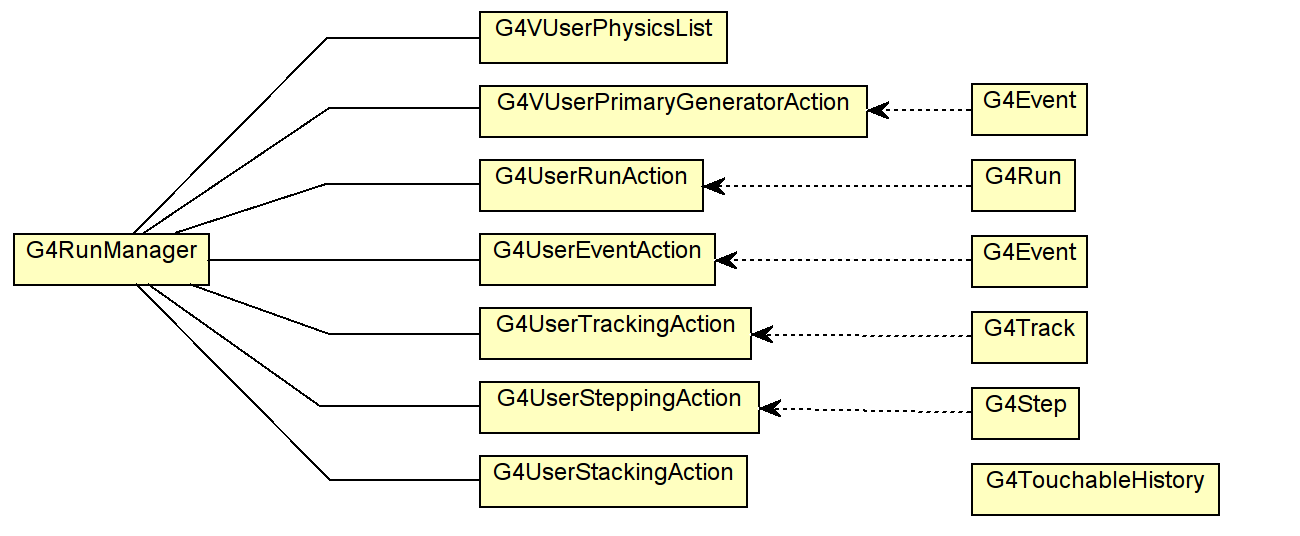
\includegraphics[height=70mm] {DDG4-G4RunManagerAnatomy.png}
    \caption{The various user hooks provided by Geant4. Not shown here
              is the callback system interfacing to the active elements
              of the detector design.}
    \label{fig:ddg4-g4runmanager-anatomy}
  \end{center}
\end{figure}

\noindent
In detail the following object-hooks allow the client to define user provided actions:
\begin{itemize}\itemcompact
\item The \bold{User Physics List} allows the client to customize and define 
    the underlying physics process(es) which define the particle interactions 
    inside the detector defined with the geometry description.
    These interactions define the detector response in terms of 
    energy depositions.
\item The \bold{Run Action} is called once at the start and end of a run. 
    i.e. a series of generated events. These two callbacks
    allow clients to define run-dependent actions such as statistics
    summaries etc.
\item The \bold{Primary Generator Action} is called for every event.
    During the callback all particles are created which form the 
    microscopic kinematic action of the particle collision.
    This input may either origin directly from an event generator program
    or come from file.
\item The \bold{Event Action} is called once at the start and the end of each event.
     It is typically used for a simple analysis of the processed event.
     If the simulated data should be written to some persistent medium, 
     the call at the end of the event processing is the appropriate place.
\item The \bold{Tracking Action} 
\item The \bold{Stepping Action} 
\item The \bold{Stacking Action} 
\end{itemize}
\noindent
Geant4 provides all callbacks with the necessary information in the form of 
appropriate arguments.

\noindent
Besides the callback system, Geant4 provides callbacks whenever a particle
traverses a sensitive volume. These callbacks are called 
- similar to event actions - once at the start and the end of the event,
but in addition, if either the energy deposit of a particle in the 
sensitive volume exceeds some threshold. The callbacks are formalized within 
the base class \tts{G4VSensitiveDetector}.

\input{DDG4Manual-Implementation.tex}

%=============================================================================
\section{Setting up DDG4}
\label{sec:ddg4-implementation-setup}
%=============================================================================

\noindent
\DDG offers several possibilities to configure a simulation application
using
\begin{itemize}\itemcompact
\item XML files,
\item by coding a setup script loaded from the \tts{ROOT} interpreter 
	with the AClick	mechanism.
\item by creating a setup script using \tts{python} and 
	\tts{ROOT}'s reflection mechanism exposed by \tts{PyROOT}.
\end{itemize}
The following subsection describe these different mechanism. An attempt was made
to match the naming conventions of all approaches where possible.

%=============================================================================
\subsection{Setting up DDG4 using XML}
\label{sec:ddg4-implementation-setup-xml}
%=============================================================================

\noindent
A special plugin was developed to enable the configuration of \DDG using
XML structures. These files are parsed identically to the geometry setup
in \DDhep the only difference is the name of the root-element, which for 
\DDG is \tts{<geant4\_setup>}. 
The following code snippet shows the basic structure of a \DDG setup file:
\begin{unnumberedcode}
<geant4_setup>
  <physicslist>          ,,,  </physicslist>  <!-- Definition of the physics list          -->
  <actions>              ...  </actions>      <!-- The list of global actions              -->
  <phases>               ...  </phases>       <!-- The definition of the various phases    -->
  <filters>              ...  </filters>      <!-- The list of global filter actions       -->
  <sequences>            ...  </sequences>    <!-- The list of defined sequences           -->
  <sensitive_detectors>  ...  </sensitive_detectors>  <!-- The list of sensitive detectors -->
  <properties>           ...  </properties>   <!-- Free format option sequences            -->
</geant4_setup>
\end{unnumberedcode}
To setup a \DDG4 application any number of xml setup files may be interpreted 
iteratively. In the following subsections the content of these first level sub-trees will
be discussed.

%=============================================================================
\subsubsection{Setup of the Physics List}
\label{sec:ddg4-setup-xml-physicslist}
%=============================================================================

\noindent
The main tag to setup a physics list is \tts{<physicslist>} with the 
\tts{name} attribute defining the instance of the \tts{Geant4PhysicsList} object.
An example code snippet is shown below in Figure~\ref{fig:ddg4-setup-xml-physicslist}.

\begin{code}
<geant4_setup>
  <physicslist name="Geant4PhysicsList/MyPhysics.0">

    <extends name="QGSP_BERT"/>                    <!-- Geant4 basic Physics list -->

    <particles>                                    <!-- Particle constructors     -->
      <construct name="G4Geantino"/>
      <construct name="G4ChargedGeantino"/>
      <construct name="G4Electron"/>
      <construct name="G4Gamma"/>
      <construct name="G4BosonConstructor"/>
      <construct name="G4LeptonConstructor"/>
      <construct name="G4MesonConstructor"/>
      <construct name="G4BaryonConstructor"/>
      ...
    </particles>

    <processes>                                    <!-- Process constructors      -->
      <particle name="e[+-]" cut="1*mm">
        <process name="G4eMultipleScattering"  ordAtRestDoIt="-1"       ordAlongSteptDoIt="1"
                                               ordPostStepDoIt="1"/>
        <process name="G4eIonisation"          ordAtRestDoIt="-1"       ordAlongSteptDoIt="2"
                                               ordPostStepDoIt="2"/>
      </particle>
      <particle name="mu[+-]">
        <process name="G4MuMultipleScattering" ordAtRestDoIt="-1"       ordAlongSteptDoIt="1"     
                                               ordPostStepDoIt="1"/>
        <process name="G4MuIonisation"         ordAtRestDoIt="-1"       ordAlongSteptDoIt="2"
                                               ordPostStepDoIt="2"/>
      </particle>
      ...
    </processes>

    <physics>                                      <!-- Physics constructors      -->
      <construct name="G4EmStandardPhysics"/>
      <construct name="HadronPhysicsQGSP"/>
      ...
    </physics>
    
  </physicslist>
</geant4_setup>
\end{code}
\begin{figure}[h]
\caption{XML snippet showing the configuration of a physics list.}
\label{fig:ddg4-setup-xml-physicslist}
\end{figure}

\begin{itemize}\itemcompact
\item To base all these constructs on an already existing predefined Geant4 physics list
    use the \tts{<extends>} tag with the attribute containing the name of the physics list
    as shown in line 4.
\item To trigger a call to a \bold{particle constructors} (line 7-14), use the \tts{<particles>} section 
    and define the Geant4 particle constructor to be called by name. To trigger a call to
\item \bold{physics process constructors}, as shown in line 19-30, 
    Define for each particle matching the name pattern (regular expression!) and the 
    default cut value for the corresponding processes. The attributes ordXXXX correspond
    to the arguments of the Geant4 call \\
    \tts{G4ProcessManager::AddProcess(process,ordAtRestDoIt, ordAlongSteptDoIt,ordPostStepDoIt);}
    The processes themself are created using the ROOT plugin mechanism.
    To trigger a call to
\item \bold{physics constructors}, as shown in line 34-35, use the \tts{<physics>} section.
\end{itemize}
If only a predefined physics list is used, which probably already satisfies very many use cases,
all these section collapse to:
\begin{code}
<geant4_setup>
  <physicslist name="Geant4PhysicsList/MyPhysics.0">
    <extends name="QGSP_BERT"/>                    <!-- Geant4 basic Physics list -->
  </physicslist>
</geant4_setup>
\end{code}

%=============================================================================
\subsubsection{Setup of Global Geant4 Actions}
\label{sec:ddg4-setup-xml-geant4-actions}
%=============================================================================

\noindent
Global actions must be defined in the \tts{<actions>} section as shown in the following snippet:
\begin{code}
<geant4_setup>
  <actions>
    <action name="Geant4TestRunAction/RunInit">
      <properties Property_int="12345"
          Property_double="-5e15"
          Property_string="Startrun: Hello_2"/>
     </action>
    <action name="Geant4TestEventAction/UserEvent_2"
            Property_int="1234"
            Property_double="5e15"
            Property_string="Hello_2" />
  </actions>
</geant4_setup>
\end{code}
The default properties of \bold{every} \tts{Geant4Action} object are:
\begin{unnumberedcode}
Name        [string]                Action name
OutputLevel [int]                   Flag to customize the level of printout
Control     [boolean]               Flag if the UI messenger should be installed.
\end{unnumberedcode}
The \tts{name} attribute of an action child is a qualified name: The first part
denotes the type of the plugin (i.e. its class), the second part the name of the instance.
Within one collection the instance \tts{name} must be unique.
Properties of Geant4Actions are set by placing them as attributes into the
\tts{<properties>} section.

%=============================================================================
\subsubsection{Setup of Geant4 Filters}
\label{sec:ddg4-setup-xml-geant4-filters}
%=============================================================================
\noindent
Filters are special actions called by \tts{Geant4Sensitive}s. 
Filters may be global or anonymous i.e. reusable by several sensitive detector
sequences as illustrated in Section~\ref{sec:ddg4-setup-xml-geant4-sequences}. 
The setup is analogous to the setup of global actions:
\begin{code}
  <filters>
    <filter name="GeantinoRejectFilter/GeantinoRejector"/>
    <filter name="ParticleRejectFilter/OpticalPhotonRejector">
      <properties particle="opticalphoton"/>
    </filter>
    <filter name="ParticleSelectFilter/OpticalPhotonSelector">
      <properties particle="opticalphoton"/>
    </filter>
    <filter name="EnergyDepositMinimumCut">
      <properties Cut="10*MeV"/>
    </filter>
    <!--        ... next global filter ...       -->
  </filters>
\end{code}
Global filters are accessible from the \tts{Geant4Kernel} object.

%=============================================================================
\subsubsection{Geant4 Action Sequences}
\label{sec:ddg4-setup-xml-geant4-sequences}
%=============================================================================

\noindent
\tts{Geant4 Action Sequences} by definition are \tts{Geant4Action} objects.
Hence, they share the setup mechanism with properties etc. For the setup
mechanism two different types of sequences are known to \DDG:
{\it{Action sequences}} and {\it{Sensitive detector sequences}}. Bot are declared in
the \tts{sequences} section:
\begin{code}
<geant4_setup>
  <sequences>
    <sequence name="Geant4EventActionSequence/EventAction"> <!-- Sequence "EventAction" of type
                                                                 "Geant4EventActionSequence" -->
      <action name="Geant4TestEventAction/UserEvent_1">     <!-- Anonymous action                   -->
        <properties Property_int="01234"                    <!-- Properties go inline               -->
            Property_double="1e11"
            Property_string="'Hello_1'"/>
      </action>
      <action name="UserEvent_2"/>                          <!-- Global action defined in "actions" -->
                                                            <!-- Only the name is referenced here   -->
      <action name="Geant4Output2ROOT/RootOutput">          <!-- ROOT I/O action                    -->
        <properties Output="simple.root"/>                  <!-- Output file property               -->
      </action>
      <action name="Geant4Output2LCIO/LCIOOutput">          <!-- LCIO output action                 -->
        <properties Output="simple.lcio"/>                  <!-- Output file property               -->
      </action>
    </sequence>


    <sequence sd="SiTrackerBarrel" type="Geant4SensDetActionSequence">
      <filter name="GeantinoRejector"/>
      <filter name="EnergyDepositMinimumCut"/>
      <action name="Geant4SimpleTrackerAction/SiTrackerBarrelHandler"/>
    </sequence>
    <sequence sd="SiTrackerEndcap" type="Geant4SensDetActionSequence">
      <filter name="GeantinoRejector"/>
      <filter name="EnergyDepositMinimumCut"/>
      <action name="Geant4SimpleTrackerAction/SiTrackerEndcapHandler"/>
    </sequence>
    <!--    ... next sequence ...     -->
  </sequences>
</geant4_setup>
\end{code}
Here firstly the \bold{EventAction} sequence is defined with its members. 
Secondly a sensitive detector sequence is defined for the subdetector
\tts{SiTrackerBarrel} of type \tts{Geant4SensDetActionSequence}.
The sequence uses two filters: \tts{GeantinoRejector} to not generate hits
from geantinos and \tts{EnergyDepositMinimumCut} to enforce a minimal energy deposit.
These filters are global i.e. they may be applied by many subdetectors.
The setup of global filters is described in 
Section~\ref{sec:ddg4-setup-xml-geant4-filters}.
Finally the action \tts{SiTrackerEndcapHandler} of type \tts{Geant4SimpleTrackerAction}
is chained, which collects the deposited energy and 
creates a collection of hits. The \tts{Geant4SimpleTrackerAction} is a template
callback to illustrate the usage of sensitive elements in \DDG.
The resulting hit collection of these handlers by default have the same name as the
object instance name.
Analogous below the sensitive detector sequence for the subdetector 
\tts{SiTrackerEndcap} is shown, which reuses the same filter actions, but will build its own
hit collection.

\noindent
\bold{Please note:}
\begin{itemize}\itemcompact
\item \bold{It was already mentioned, but once again}: Event-, run-, generator-, tracking-,
    stepping- and stacking actions sequences have predefined names! 
    These names are fixed and part of the \bold{common knowledge}, they cannot be altered.
    Please refer to 
    Section~\ref{sec:ddg4-user-manual-implementation-geant4action-sequences} 
    for the names of the global action sequences.
\item the sensitive detector sequences are matched by the attribute \tts{sd} to the 
    subdetectors created with the \DDhep detector description package. Values must match!
\item In the event that several xml files are parsed it is absolutely vital that 
    the \tts{<actions>} section is interpreted \bold{before} the \tts{sequences}.
\item For each XML file several \tts{<sequences>} are allowed.
\noindent
\end{itemize}

%=============================================================================
\subsubsection{Setup of Geant4 Sensitive Detectors}
\label{sec:ddg4-setup-xml-geant4-sensitive detectors}
%=============================================================================
\begin{code}
  <geant4_setup>
    <sensitive_detectors>
      <sd name="SiTrackerBarrel" 
          type="Geant4SensDet" 
          ecut="10.0*MeV" 
          verbose="true" 
          hit_aggregation="position">
      </sd>
      <!-- ...  next sensitive detector ... -->
    </sensitive_detectors>
  </geant4_setup>
\end{code}



%=============================================================================
\subsubsection{Miscellaneous Setup of Geant4 Objects}
\label{sec:ddg4-setup-xml-geant4-objects}
%=============================================================================

\noindent
This section is used for the flexible setup of auxiliary objects such as the 
electromagnetic fields used in Geant4:
\begin{code}
  <geant4_setup>
    <properties>
      <attributes name="geant4_field"
            id="0"
            type="Geant4FieldSetup"
            object="GlobalSolenoid"
            global="true"
            min_chord_step="0.01*mm"
            delta_chord="0.25*mm"
            delta_intersection="1e-05*mm"
            delta_one_step="0.001*mm"
            eps_min="5e-05*mm"
            eps_max="0.001*mm"
            largest_step = "10*m"
            stepper="HelixSimpleRunge"
            equation="Mag_UsualEqRhs">
      </attributes>
      ...
    </properties>
  </geant4_setup>
\end{code}
Important are the tags \tts{type} and \tts{object}, which are used to firstly
define the plugin to be called and secondly define the object from the \DDhep
description to be configured for the use within Geant4.

%=============================================================================
\subsubsection{Setup of Geant4 Phases}
\label{sec:ddg4-setup-xml-geant4-phases}
%=============================================================================

\noindent
Phases are configured as shown below.
However, the use is \bold{discouraged},
since it is not yet clear if there are appropriate use cases!
\begin{code}
  <phases>
    <phase type="RunAction/begin">
      <action name="RunInit"/>
      <action name="Geant4TestRunAction/UserRunInit">
    <properties Property_int="1234"
            Property_double="5e15"
            Property_string="'Hello_2'"/>
      </action>
    </phase>
    <phase type="EventAction/begin">
      <action name="UserEvent_2"/>
    </phase>
    <phase type="EventAction/end">
      <action name="UserEvent_2"/>
    </phase>
    ...
  </phases>
\end{code}

\newpage
%=============================================================================
\subsection{Setting up DDG4 using ROOT-CINT}
\label{sec:ddg4-implementation-setup-root-cint}
%=============================================================================

\noindent
The setup of \DDG directly from the the ROOT interpreter using the AClick
mechanism is very simple, but mainly meant for purists (like me ;-)),
since it is nearly equivalent to the explicit setup within a \tts{C++} 
main program.
The following code section shows how to do it. For explanation the code
segment is discussed below line by line.
\begin{code}
#include "DDG4/Geant4Config.h"
#include "DDG4/Geant4TestActions.h"
#include "DDG4/Geant4TrackHandler.h"
#include <iostream>

using namespace std;
using namespace dd4hep;
using namespace dd4hep::sim;
using namespace dd4hep::sim::Test;
using namespace dd4hep::sim::Setup;

#if defined(__MAKECINT__)
#pragma link C++ class Geant4RunActionSequence;
#pragma link C++ class Geant4EventActionSequence;
#pragma link C++ class Geant4SteppingActionSequence;
#pragma link C++ class Geant4StackingActionSequence;
#pragma link C++ class Geant4GeneratorActionSequence;
#pragma link C++ class Geant4Action;
#pragma link C++ class Geant4Kernel;
#endif

SensitiveSeq::handled_type* setupDetector(Kernel& kernel, const std::string& name)   {
  SensitiveSeq sd = SensitiveSeq(kernel,name);
  Sensitive  sens = Sensitive(kernel,"Geant4TestSensitive/"+name+"Handler",name);
  sd->adopt(sens);
  sens = Sensitive(kernel,"Geant4TestSensitive/"+name+"Monitor",name);
  sd->adopt(sens);
  return sd;
}

void exampleAClick()  {
  Geant4Kernel& kernel = Geant4Kernel::instance(Detector::getInstance());
  kernel.loadGeometry("file:../DD4hep.trunk/DDExamples/CLICSiD/compact/compact.xml");
  kernel.loadXML("DDG4_field.xml");

  GenAction gun(kernel,"Geant4ParticleGun/Gun");
  gun["energy"] = 0.5*GeV;                          // Set properties
  gun["particle"] = "e-";
  gun["multiplicity"] = 1;
  kernel.generatorAction().adopt(gun);

  Action run_init(kernel,"Geant4TestRunAction/RunInit");
  run_init["Property_int"] = 12345;
  kernel.runAction().callAtBegin  (run_init.get(),&Geant4TestRunAction::begin);
  kernel.eventAction().callAtBegin(run_init.get(),&Geant4TestRunAction::beginEvent);
  kernel.eventAction().callAtEnd  (run_init.get(),&Geant4TestRunAction::endEvent);

  Action evt_1(kernel,"Geant4TestEventAction/UserEvent_1");
  evt_1["Property_int"] = 12345;                    // Set properties
  evt_1["Property_string"] = "Events";
  kernel.eventAction().adopt(evt_1);

  EventAction evt_2(kernel,"Geant4TestEventAction/UserEvent_2");
  kernel.eventAction().adopt(evt_2);

  kernel.runAction().callAtBegin(evt_2.get(),&Geant4TestEventAction::begin);
  kernel.runAction().callAtEnd  (evt_2.get(),&Geant4TestEventAction::end);
 
  setupDetector(kernel,"SiVertexBarrel");
  setupDetector(kernel,"SiVertexEndcap");
  // .... more subdetectors here .....
  setupDetector(kernel,"LumiCal");
  setupDetector(kernel,"BeamCal");

  kernel.configure();
  kernel.initialize();
  kernel.run();
  std::cout << "Successfully executed application .... " << std::endl;
  kernel.terminate();
}
\end{code}

\noindent
\begin{tabular} {l||p{0cm}}
\docline{Line}{}
\docline{1}{The header file \tts{Geant4Config.h} contains a set of wrapper
    classes to easy the creation of objects using the plugin mechanism and setting
    properties to \tts{Geant4Action} objects. These helpers and the corresponding 
    functionality are not included in the wrapped classes themselves to not 
    clutter the code with stuff only used for the setup.
    All contained objects are in the namespace \tts{dd4hep::sim::Setup}}.
\docline{6-10}{Save yourself specifying all the namespaces objects are in....}
\docline{13-19}{CINT processing pragmas. 
    Classes defined here will be available at the ROOT prompt
    after this AClick is loaded.}
\docline{22-29}{Sampler to fill the sensitive detector sequences for each 
    subdetector with two entries: a handler and a monitor action.
    Please note, that this here is example code and in real life specialized actions
    will have to be provided for each subdetector.}
\docline{31}{Let's go for it. here the entry point starts....}
\docline{32}{Create the \tts{Geant4Kernel} object.}
\docline{33}{Load the geometry into \DDhep.}
\docline{34}{Redefine the setup of the sensitive detectors.}
\docline{36-40}{Create the generator action of type \tts{Geant4ParticleGun} with name
    \tts{Gun}, set non-default properties and activate the configured object
    by attaching it to the \tts{Geant4Kernel}.}
\docline{42-46}{Create a user defined begin-of-run action callback, set the properties
    and attach it to the begin of run calls. To collect statistics extra member functions
    are registered to be called at the beginning and the end of each event.}
\docline{48-51}{Create a user defined event action routine, set its properties
    and attach it to the event action sequence.}
\docline{53-54}{Create a second event action and register it to the event action sequence.
    This action will be called after the previously created action.}
\docline{56-57}{For this event action we want to receive callbacks at start- 
    and end-of-run to produce additional summary output.}
\docline{59-63}{Call the sampler routine to attach test actions to the subdetectors defined.}
\docline{65-66}{Configure, initialize and run the Geant4 application.
    Most of the Geant4 actions will only be created here and the action sequences
    created before will be attached now.}
\docline{69}{Terminate the Geant4 application and exit.}
\end{tabular}

\newpage
\noindent
CINT currently cannot handle pointers to member functions~\footnote{This may change
in the future once ROOT uses \tts{clang} and \tts{cling} as the interpreting engine.}. 
Hence the above AClick only works in compiled mode. To invoke the compilation the following 
action is necessary from the ROOT prompt:


\begin{code}
$> root.exe
  *******************************************
  *                                         *
  *        W E L C O M E  to  R O O T       *
  *                                         *
  *   Version   5.34/10    29 August 2013   *
  *                                         *
  *  You are welcome to visit our Web site  *
  *          http://root.cern.ch            *
  *                                         *
  *******************************************

ROOT 5.34/10 (heads/v5-34-00-patches@v5-34-10-5-g0e8bac8, Sep 04 2013, 11:52:19 on linux)

CINT/ROOT C/C++ Interpreter version 5.18.00, July 2, 2010
Type ? for help. Commands must be C++ statements.
Enclose multiple statements between { }.
root [0] .X initAClick.C
.... Setting up the CINT include pathes and the link statements.

root [1] .L ../DD4hep.trunk/DDG4/examples/exampleAClick.C+
Info in <TUnixSystem::ACLiC>: creating shared library ....exampleAClick_C.so
.... some Cint warnings concerning member function pointers .....

root [2] exampleAClick()
.... and it starts ...
\end{code}

\noindent
The above scripts are present in the DDG4/example directory located in svn.
The initialization script \tts{initAClick.C} may require customization
to cope with the installation paths.

%=============================================================================
\subsection{Setting up DDG4 using Python}
\label{sec:ddg4-implementation-setup-python}
%=============================================================================

\noindent
Given the reflection interface of ROOT, the setup of the simulation interface
using dd4hep is of course also possible using the python interpreted language.
In the following code example the setup of Geant4 using the \tts{ClicSid} 
example is shown using python~\footnote{For comparison, the same example was 
used to illustrate the setup using XML files.}.

\begin{code}
import DDG4
from SystemOfUnits import *

"""

   dd4hep example setup using the python configuration

   @author  M.Frank
   @version 1.0

"""
def run():
  kernel = DDG4.Kernel()
  kernel.loadGeometry("file:../DD4hep.trunk/DDExamples/CLICSiD/compact/compact.xml")
  kernel.loadXML("DDG4_field.xml")

  description = kernel.detectorDescription()
  print '+++   List of sensitive detectors:'
  for i in description.detectors(): 
    o = DDG4.DetElement(i.second)
    sd = description.sensitiveDetector(o.name())
    if sd.isValid():
      print '+++  %-32s type:%s'%(o.name(), sd.type(), )

  # Configure Run actions
  run1 = DDG4.RunAction(kernel,'Geant4TestRunAction/RunInit')
  run1.Property_int    = 12345
  run1.Property_double = -5e15*keV
  run1.Property_string = 'Startrun: Hello_2'
  print run1.Property_string, run1.Property_double, run1.Property_int
  run1.enableUI()
  kernel.registerGlobalAction(run1)
  kernel.runAction().add(run1)

  # Configure Event actions
  evt2 = DDG4.EventAction(kernel,'Geant4TestEventAction/UserEvent_2')
  evt2.Property_int    = 123454321
  evt2.Property_double = 5e15*GeV
  evt2.Property_string = 'Hello_2 from the python setup'
  evt2.enableUI()
  kernel.registerGlobalAction(evt2)

  evt1 = DDG4.EventAction(kernel,'Geant4TestEventAction/UserEvent_1')
  evt1.Property_int=01234
  evt1.Property_double=1e11
  evt1.Property_string='Hello_1'
  evt1.enableUI()

  kernel.eventAction().add(evt1)
  kernel.eventAction().add(evt2)

  # Configure I/O
  evt_root = DDG4.EventAction(kernel,'Geant4Output2ROOT/RootOutput')
  evt_root.Control = True
  evt_root.Output = "simple.root"
  evt_root.enableUI()

  evt_lcio = DDG4.EventAction(kernel,'Geant4Output2LCIO/LcioOutput')
  evt_lcio.Output = "simple_lcio"
  evt_lcio.enableUI()

  kernel.eventAction().add(evt_root)
  kernel.eventAction().add(evt_lcio)

  # Setup particle gun
  gun = DDG4.GeneratorAction(kernel,"Geant4ParticleGun/Gun")
  gun.energy   = 0.5*GeV
  gun.particle = 'e-'
  gun.multiplicity = 1
  gun.enableUI()
  kernel.generatorAction().add(gun)

  # Setup global filters for use in sensitive detectors
  f1 = DDG4.Filter(kernel,'GeantinoRejectFilter/GeantinoRejector')
  f2 = DDG4.Filter(kernel,'ParticleRejectFilter/OpticalPhotonRejector')
  f2.particle = 'opticalphoton'
  f3 = DDG4.Filter(kernel,'ParticleSelectFilter/OpticalPhotonSelector') 
  f3.particle = 'opticalphoton'
  f4 = DDG4.Filter(kernel,'EnergyDepositMinimumCut')
  f4.Cut = 10*MeV
  f4.enableUI()
  kernel.registerGlobalFilter(f1)
  kernel.registerGlobalFilter(f2)
  kernel.registerGlobalFilter(f3)
  kernel.registerGlobalFilter(f4)

  # First the tracking detectors
  seq = DDG4.SensitiveSequence(kernel,'Geant4SensDetActionSequence/SiVertexBarrel')
  act = DDG4.SensitiveAction(kernel,'Geant4SimpleTrackerAction/SiVertexBarrelHandler','SiVertexBarrel')
  seq.add(act)
  seq.add(f1)
  seq.add(f4)
  act.add(f1)

  seq = DDG4.SensitiveSequence(kernel,'Geant4SensDetActionSequence/SiVertexEndcap')
  act = DDG4.SensitiveAction(kernel,'Geant4SimpleTrackerAction/SiVertexEndcapHandler','SiVertexEndcap')
  seq.add(act)
  seq.add(f1)
  seq.add(f4)

  seq = DDG4.SensitiveSequence(kernel,'Geant4SensDetActionSequence/SiTrackerBarrel')
  act = DDG4.SensitiveAction(kernel,'Geant4SimpleTrackerAction/SiTrackerBarrelHandler','SiTrackerBarrel')
  seq.add(act)
  seq.add(f1)
  seq.add(f4)

  seq = DDG4.SensitiveSequence(kernel,'Geant4SensDetActionSequence/SiTrackerEndcap')
  act = DDG4.SensitiveAction(kernel,'Geant4SimpleTrackerAction/SiTrackerEndcapHandler','SiTrackerEndcap')
  seq.add(act)

  seq = DDG4.SensitiveSequence(kernel,'Geant4SensDetActionSequence/SiTrackerForward')
  act = DDG4.SensitiveAction(kernel,'Geant4SimpleTrackerAction/SiTrackerForwardHandler','SiTrackerForward')
  seq.add(act)

  # Now the calorimeters
  seq = DDG4.SensitiveSequence(kernel,'Geant4SensDetActionSequence/EcalBarrel')
  act = DDG4.SensitiveAction(kernel,'Geant4SimpleCalorimeterAction/EcalBarrelHandler','EcalBarrel')
  seq.add(act)

  seq = DDG4.SensitiveSequence(kernel,'Geant4SensDetActionSequence/EcalEndcap')
  act = DDG4.SensitiveAction(kernel,'Geant4SimpleCalorimeterAction/EcalEndCapHandler','EcalEndcap')
  seq.add(act)

  seq = DDG4.SensitiveSequence(kernel,'Geant4SensDetActionSequence/HcalBarrel')
  act = DDG4.SensitiveAction(kernel,'Geant4SimpleCalorimeterAction/HcalBarrelHandler','HcalBarrel')
  act.adoptFilter(kernel.globalFilter('OpticalPhotonRejector'))
  seq.add(act)

  act = DDG4.SensitiveAction(kernel,'Geant4SimpleCalorimeterAction/HcalOpticalBarrelHandler','HcalBarrel')
  act.adoptFilter(kernel.globalFilter('OpticalPhotonSelector'))
  seq.add(act)

  seq = DDG4.SensitiveSequence(kernel,'Geant4SensDetActionSequence/HcalEndcap')
  act = DDG4.SensitiveAction(kernel,'Geant4SimpleCalorimeterAction/HcalEndcapHandler','HcalEndcap')
  seq.add(act)

  seq = DDG4.SensitiveSequence(kernel,'Geant4SensDetActionSequence/HcalPlug')
  act = DDG4.SensitiveAction(kernel,'Geant4SimpleCalorimeterAction/HcalPlugHandler','HcalPlug')
  seq.add(act)

  seq = DDG4.SensitiveSequence(kernel,'Geant4SensDetActionSequence/MuonBarrel')
  act = DDG4.SensitiveAction(kernel,'Geant4SimpleCalorimeterAction/MuonBarrelHandler','MuonBarrel')
  seq.add(act)

  seq = DDG4.SensitiveSequence(kernel,'Geant4SensDetActionSequence/MuonEndcap')
  act = DDG4.SensitiveAction(kernel,'Geant4SimpleCalorimeterAction/MuonEndcapHandler','MuonEndcap')
  seq.add(act)

  seq = DDG4.SensitiveSequence(kernel,'Geant4SensDetActionSequence/LumiCal')
  act = DDG4.SensitiveAction(kernel,'Geant4SimpleCalorimeterAction/LumiCalHandler','LumiCal')
  seq.add(act)

  seq = DDG4.SensitiveSequence(kernel,'Geant4SensDetActionSequence/BeamCal')
  act = DDG4.SensitiveAction(kernel,'Geant4SimpleCalorimeterAction/BeamCalHandler','BeamCal')
  seq.add(act)

  # Now build the physics list:
  phys = kernel.physicsList()
  phys.extends = 'FTFP_BERT'
  #phys.transportation = True
  phys.decays  = True
  phys.enableUI()

  ph = DDG4.PhysicsList(kernel,'Geant4PhysicsList/Myphysics')
  ph.addParticleConstructor('G4BosonConstructor')
  ph.addParticleConstructor('G4LeptonConstructor')
  ph.addParticleProcess('e[+-]','G4eMultipleScattering',-1,1,1)
  ph.addPhysicsConstructor('G4OpticalPhysics')
  ph.enableUI()
  phys.add(ph)

  phys.dump()

  kernel.configure()
  kernel.initialize()
  kernel.run()
  kernel.terminate()

if __name__ == "__main__":
  run()

\end{code}

\newpage
%=============================================================================
\subsection{A Simple Example}
\label{sec:ddg4-implementation-simple-example}
%=============================================================================
\noindent
Bla-bal.

\newpage


\input{DDG4Manual-HighLevel.tex}

%=============================================================================
\section{Multi-Threading in \DDG}
\label{sec:ddg4-multi-threading}
%=============================================================================
\subsection{Introductory Remarks}
\label{sec:ddg4-multi-threading-introduction}
%=============================================================================
\noindent
Multi-threading as supported by Geant4 is event driven. This means that 
the simulation of a given event is handled by one single thread.
Geant4 provides specific extensions to ease the users the use of its 
multi-threaded extensions~\cite{bib:Geant4-multi-threading}~\footnote{Please
note that the whole of Geant4 and your client code must be compiled with
the compile flag ${\tts{-DGEANT4_BUILD_MULTITHREADED=ON}}$}.
These extension divide in a formalized manner all actions to be performed
to setup a Geant4 multi-threaded program into

\begin{itemize}\itemcompact
\item {\bf{common}} actions to be performed and shared by all threads.
This includes the setup of the geometry and the physics list. The
other main area are
\item {\bf{thread-specific}} actions to be performed for each thread.
These are composed by the user actions called during the processing of
each run. These are the run-, event-, generation-, tracking-, 
stepping and stacking actions.
\end{itemize}

\noindent
To understand the interplay between \DDG and Geant4 let us quickly 
recapitulate the Geant4 mechanism how to configure multiple threads.
The setup of a multi-threaded application in Geant4 is centered around 
two additional classes, which both deal with single- and multi-threaded 
issues:

\begin{itemize}\itemcompact
\item {\tts{G4VUserActionInitialization}} class with 2 major callbacks:
	{\tts{Build()}} which is executed for each {\bf{worker thread}} and 
	{\tts{BuildForMaster()}} which is executed for master thread only.	
\item {\tts{G4VUserDetectorConstruction}} class with the callbacks
    {\tts{Construct()}}, where the shared geometry is constructed and
    {\tts{ConstructSDandField()}} where the sensitive detectors and the
    electro magnetic fields are provided.
\end{itemize}

\noindent
Both these Geant4 provided hooks are modeled in the standard \DDG 
way as action queues, which allow a modular and fine grained setup
as shown in Figure~\ref{fig:ddg4-user-initialization} and 
Figure~\ref{fig:ddg4-detector-initialization}.
\begin{figure}[t]
  \begin{center}
    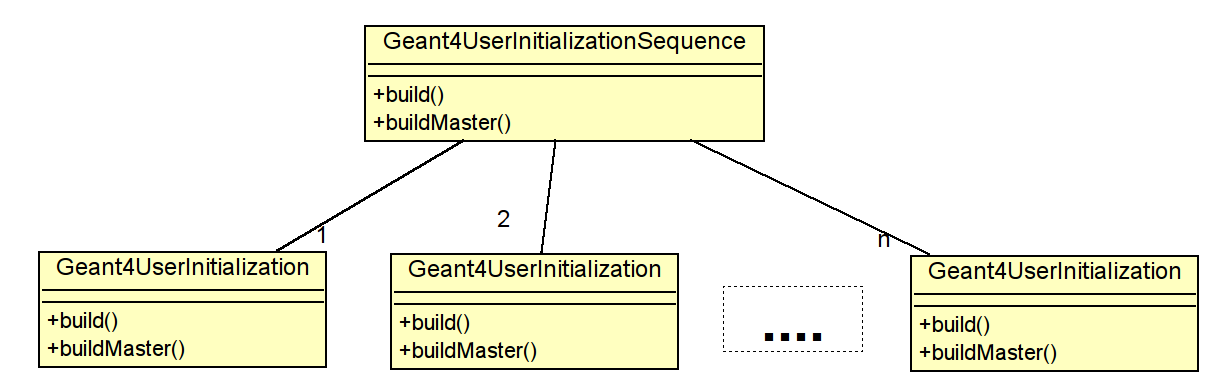
\includegraphics[width=140mm] {DDG4-User-Initialization.png}
    \caption{The Geant4 user initialization sequence to setup DDG4
             in multi-threaded mode. The callbacks {\tts{buildMaster()}} 
             is only called in multi-threaded mode.}
    \label{fig:ddg4-user-initialization}
  \end{center}
\end{figure}

\noindent
The \DDG framework ensures that all user callbacks are installed properly
to the Geant4 run manager, which calls them appropriately at the correct time.

\noindent
\DDG provides three callbacks for each sequence. Each callback receives
a temporary context argument, which may be used to shortcut access 
to basic useful quantities:
\begin{code}
    struct Geant4DetectorConstructionContext  {
      /// Reference to geometry object
      Detector&     description;
      /// Reference to the world after construction
      G4VPhysicalVolume*  world;
      /// The cached geometry information
      Geant4GeometryInfo* geometry;
      /// G4 User detector initializer
      G4VUserDetectorConstruction* detector;
};
\end{code}

\begin{figure}[h]
  \begin{center}
    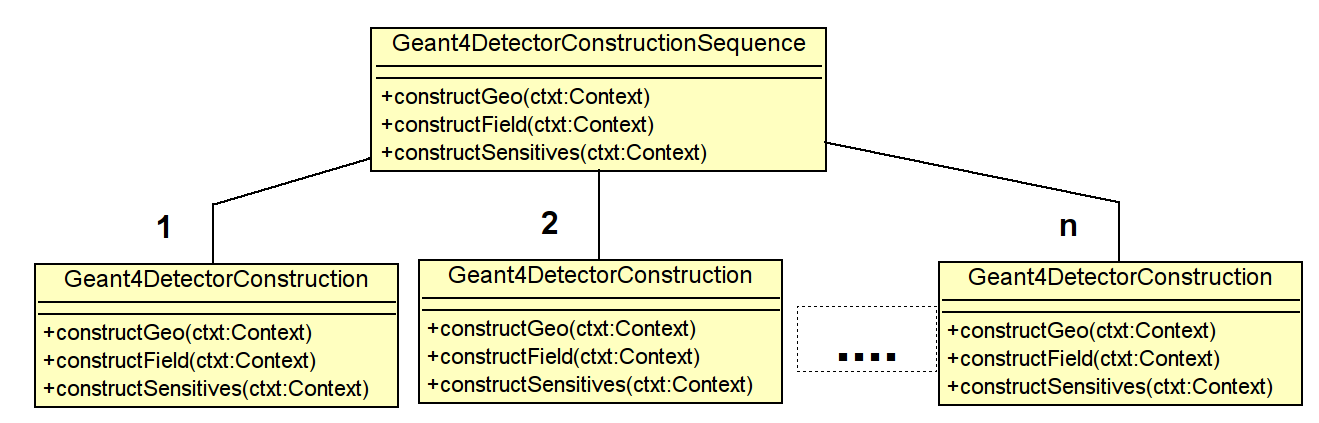
\includegraphics[width=140mm] {DDG4-Detector-Construction.png}
    \caption{The Geant4 detector initialization sequence to setup DDG4.
        If supplied, Geant4 calls the components both, in the single-threaded 
        and in the multi-threaded mode.}
    \label{fig:ddg4-detector-initialization}
  \end{center}
\end{figure}

The callbacks and the expected functionality are:
\begin{enumerate}
\item First the detector geometry is constructed. This happens in the callback
    {\tts{constructGeo(...)}}. If a standard \DDhep geometry 
    is present, this is translation of the geometry could be done by simply 
    calling the plugin {\tts{Geant4DetectorGeometryConstruction}}. 
    Alternatively a user defined plugin could perform this action.
\item Next the electromagnetic fields for the Geant4 particle tracking is
    constructed. A generic plugin {\tts{Geant4FieldTrackingConstruction}}
    may be attached. The corresponding setup parameters are listed in
    Section~\ref{sec:existing-ddg4-components}. 
    Alternatively a user defined plugin could perform this action.
\item Finally the Geant4 sensitive detectors are instantiated and attached 
    to the sensitive volumes. For generic setups the plugin
    {\tts{Geant4DetectorSensitivesConstruction}} may be attached.
    Alternatively a user defined plugin could perform this action.
\end{enumerate}

%=============================================================================
\subsection{Thread related contexts}
\label{sec:ddg4-thread-save context}
%=============================================================================
\noindent
\DDG provides thread related context, which may be accessed or modified
by user code. This context, the {\tts{Geant4Context}} and it's sub-components,
as discussed in Section~\ref{sec:ddg4-implementation-higher-level-components}
are available as separate instances for each event and as such
also independently for each worker thread. Hence, no user level locking of the 
event context is necessary in any worker thread.

%=============================================================================
\subsection{Thread-Shared Components}
\label{sec:ddg4-multi-threaded-shared-actions}
%=============================================================================
\noindent
Some actions, though executed in the context of a single thread context 
may only execute as singletons. An example would be a {\tts{GeneratorAction}},
which read input events from file. Clearly the reading of data from
file must be protected and the reading of one event in a given thread
must finish, before the next thread may take over.
Another example are data analysis components, which e.g. fill a histogram.
Typically the filling mechanism of a histogram is not thread safe and hence must
be protected.

\noindent
To solve such issues all actions, which may involve such shared 
activities, a shared action is provided, which adopts a singleton
instance and executes the relevant callbacks in a protected manner.
The shared actions execute the user component in a thread safe envelope.

\noindent
Clearly no run- or event related state in such shared actions may be
carried by the component object across callbacks. The action objects
may not be aware of the event related context outside the callback.
Default implementations for such shared actions exist for
\begin{itemize}\itemcompact
\item the {\tts{Geant4RunAction}}, where the calls to 
        {\tts{Geant4RunAction::begin}} and {\tts{Geant4RunAction::end}}
        are {\bf{globally}} locked and the sequential execution of 
        the entire sequence is ensured;
\item the {\tts{Geant4EventAction}},
\item the {\tts{Geant4TrackingAction}},
\item the {\tts{Geant4SteppingAction}} and
\item the {\tts{Geant4StackingAction}}.
\end{itemize}
In the latter cases the framework ensures thread safety, but does 
not ensure the reentrant execution order of the entire sequence.

\noindent
{\bf{General Remark:}}
\noindent
Simple callbacks registered to the run-, event, etc.-actions cannot 
be protected. These callbacks may under no circumstances use any 
event related state information of the called object.

%=============================================================================
\subsection{Backwards- and Single-Thread-Compatibility}
\label{sec:ddg4-multi-threading-backwards}
%=============================================================================
\noindent
As in the single threaded mode of Geant4, also in the multi-threaded
mode all user actions are called by an instance of the {\tts{G4RunManager}}
or a sublass thereof, the {\tts{G4MTRunManager}}~\cite{bib:Geant4-multi-threading}.

\noindent
If the recommended actions in sub-section~\ref{sec:ddg4-multi-threading-introduction}
are used to configure the Geant4 application, then in a rather transparent
way both single-threaded and multi-threaded setups can coexist simply by 
changing the concrete instance of the {\tts{G4RunManager}}. There is one
single exception: The user initialization function
{\tts{G4VUserActionInitialization::BuildForMaster()}} is {\bf{only}} executed
in multi-threaded mode. For this reason, we deprecate the usage. Try
to find solutions, without master specific setup using e.g. shared actions.

%=============================================================================
\subsection{Support for Python Setup in Multi-Threading Mode}
\label{sec:ddg4-multi-threading-python}
%=============================================================================
\noindent
The setup of \DDG in multi-threaded mode requires separate callbacks for 
the global configuration (geometry, etc.) and the configuration of the worker 
threads. In python this setup is performed within {\rm{python callable}}
objects, which are either functions or member functions of objects.
These functions may have arguments. The python specific configuration actions
\begin{itemize}\itemcompact
\item The user initialization action 
    {\tts{Geant4PythonInitialization}} allows to configure python callbacks
    for the master and the worker thread setup using the calls:
    \begin{code}
      /// Set the Detector initialization command
      void setMasterSetup(PyObject* callable, PyObject* args);
      /// Set the field initialization command
      void setWorkerSetup(PyObject* callable, PyObject* args);              \end{code}
     to be used in python as a call sequence within the master thread:
    \begin{code}
     init_seq = kernel.userInitialization(True)
     init_action = UserInitialization(kernel,'Geant4PythonInitialization/PyG4Init')
     init_action.setWorkerSetup(worker_setup_call, < worker_args > )
     init_action.setMasterSetup(master_setup_call, < master_args > )
     init_seq.adopt(init_action)                                            \end{code}
    The callback argument list $< worker\_args >$ and $< master\_args >$
    are python tuples containing all arguments expected by the callable objects
    $worker\_setup\_call$ and $master\_setup\_call$ respecyively.
    The class {\tts{Geant4PythonInitialization}} is a subclass of
    {\tts{Geant4UserInitialization}} and will call the provided functions
    according to the protocol explained earlier in this section.
    If a callback is not set, the corresponding actiion is not executed.
\item The detector construction action 
    {\tts{Geant4PythonDetectorConstruction}} is the corresponding 
    python action to populate the detector construction sequencer.
    and supports three ccallbacks:
    \begin{code}
      /// Set the Detector initialization command
      void setConstructGeo(PyObject* callable, PyObject* args);
      /// Set the field initialization command
      void setConstructField(PyObject* callable, PyObject* args);
      /// Set the sensitive detector initialization command
      void setConstructSensitives(PyObject* callable, PyObject* args);    \end{code}
    to be used in python as call sequence within the master thread:
    \begin{code}
    init_seq = self.master().detectorConstruction(True)
    init_action = DetectorConstruction(self.master(),name_type)
    init_action.setConstructGeo(geometry_setup_call, < geometry_args > )
    init_action.setConstructField(field_setup_call, < field_args > )
    init_action.setConstructSensitives(sensitives_setup_call, < sensitives_args >)
    init_seq.adopt(init_action)                                           \end{code}
    If any of the three callback is not set, the corresponding actiion is not executed.
    Hereby are $geometry\_setup\_call$, $field\_setup\_call$ and $sensitives\_setup\_call$ 
    the callable objects to configure the geometry, the tracking field 
    and the sensitive detectors.
    $< geometry\_args >$, $< field\_args >$ and $< sensitives\_args >$ are 
    the corresponding callable arguments in the form of a python tuple object.   
\end{itemize}

\noindent
All python callbacks are supposed to return the integer '1' on success.
Any other return code is assumed to be failure.

%=============================================================================
\subsection{\DDG Multi-Threading Example}
\label{sec:ddg4-multi-threading-example}
%=============================================================================
\begin{code}
"""

   dd4hep simulation example setup DDG4
   in multi-threaded mode using the python configuration

   @author  M.Frank
   @version 1.0

"""
import os, time, DDG4

def setupWorker(geant4):
  kernel = geant4.kernel()
  print '#PYTHON: +++ Creating Geant4 worker thread ....'
  print "#PYTHON:  Configure Run actions"
  run1 = DDG4.RunAction(kernel,'Geant4TestRunAction/RunInit')
    ...
  print "#PYTHON:  Configure Event actions"
  prt = DDG4.EventAction(kernel,'Geant4ParticlePrint/ParticlePrint')
  kernel.eventAction().adopt(prt)
    ...
  print "\n#PYTHON:  Configure I/O\n"
  evt_root = geant4.setupROOTOutput('RootOutput','CLICSiD_'+time.strftime('%Y-%m-%d_%H-%M'))
    ...
  gen = DDG4.GeneratorAction(kernel,"Geant4GeneratorActionInit/GenerationInit")
  kernel.generatorAction().adopt(gen)
  print "#PYTHON:  First particle generator: pi+"
  gen = DDG4.GeneratorAction(kernel,"Geant4IsotropeGenerator/IsotropPi+");
    ...
  print "#PYTHON:  Merge all existing interaction records"
  gen = DDG4.GeneratorAction(kernel,"Geant4InteractionMerger/InteractionMerger")
  kernel.generatorAction().adopt(gen)
  print "#PYTHON:  Finally generate Geant4 primaries"
  gen = DDG4.GeneratorAction(kernel,"Geant4PrimaryHandler/PrimaryHandler")
  kernel.generatorAction().adopt(gen)
  print "#PYTHON:  ....and handle the simulation particles."
  part = DDG4.GeneratorAction(kernel,"Geant4ParticleHandler/ParticleHandler")
  kernel.generatorAction().adopt(part)

  user = DDG4.Action(kernel,"Geant4TCUserParticleHandler/UserParticleHandler")
    ...
  part.adopt(user)
  print '#PYTHON: +++ Geant4 worker thread configured successfully....'
  return 1
  
def setupMaster(geant4):
  kernel = geant4.master()
  print '#PYTHON: +++ Setting up master thread for ',kernel.NumberOfThreads,' workers.'
  return 1

def setupSensitives(geant4):
  print "#PYTHON:  Setting up all sensitive detectors"
  geant4.printDetectors()
  print "#PYTHON:  First the tracking detectors"
  seq,act = geant4.setupTracker('SiVertexBarrel')
    ...
  print "#PYTHON:  Now setup the calorimeters"
  seq,act = geant4.setupCalorimeter('EcalBarrel')
    ...
  return 1

def run():
  kernel = DDG4.Kernel()
  description = kernel.detectorDescription()
  install_dir = os.environ['DD4hepINSTALL']
  DDG4.Core.setPrintFormat("%-32s %6s %s")
  kernel.loadGeometry("file:"+install_dir+"/DDDetectors/compact/SiD.xml")
  DDG4.importConstants(description)

  kernel.NumberOfThreads = 3
  geant4 = DDG4.Geant4(kernel,tracker='Geant4TrackerCombineAction')
  print "#  Configure UI"
  geant4.setupCshUI()

  print "#  Geant4 user initialization action"
  geant4.addUserInitialization(worker=setupWorker, worker_args=(geant4,),
                               master=setupMaster,master_args=(geant4,))
  print "#  Configure G4 geometry setup"
  seq,act = geant4.addDetectorConstruction("Geant4DetectorGeometryConstruction/ConstructGeo")

  print "# Configure G4 sensitive detectors: python setup callback"
  seq,act = geant4.addDetectorConstruction("Geant4PythonDetectorConstruction/SetupSD",
                                           sensitives=setupSensitives,sensitives_args=(geant4,))
  print "# Configure G4 sensitive detectors: atach'em to the sensitive volumes"
  seq,act = geant4.addDetectorConstruction("Geant4DetectorSensitivesConstruction/ConstructSD")

  print "#  Configure G4 magnetic field tracking"
  seq,field = geant4.addDetectorConstruction("Geant4FieldTrackingConstruction/MagFieldTrackingSetup")
  field.stepper            = "HelixGeant4Runge"
  field.equation           = "Mag_UsualEqRhs"
  field.eps_min            = 5e-05 * mm
  ...
  print "#  Setup random generator"
  rndm = DDG4.Action(kernel,'Geant4Random/Random')
  rndm.Seed = 987654321
  rndm.initialize()
  print "#  Now build the physics list:"
  phys = geant4.setupPhysics('QGSP_BERT')
  geant4.run()

if __name__ == "__main__":
  run()
\end{code}

\newpage
\input{DDG4Manual-Components.tex}

%=============================================================================
\newpage
\begin{thebibliography}{9}
\bibitem{bib:DD4hep}  DD4Hep web page, http://aidasoft.web.cern.ch/DD4hep.

\bibitem{bib:LHCb} 		LHCb Collaboration, 
                "LHCb, the Large Hadron Collider beauty experiment, reoptimised detector 
				design and performance", CERN/LHCC 2003-030

\bibitem{bib:LHCb-geometry} S. Ponce et al., 
                "Detector Description Framework in LHCb", 
                International Conference on Computing in High Energy and Nuclear Physics  (CHEP 2003), 
                La Jolla, CA, 2003, proceedings. 

\bibitem{bib:ILD}  The ILD Concept Group, 
                   "The International Large Detector: Letter of Intent",\\
                   ISBN 978-3-935702-42-3, 2009.

\bibitem{bib:SiD}  H. Aihara, P. Burrows, M. Oreglia (Editors),
                   "SiD Letter of Intent",
                   arXiv:0911.0006, 2009.

\bibitem{bib:ROOT-tgeo} R.Brun, A.Gheata, M.Gheata, "The ROOT geometry package",\\
                    Nuclear Instruments and Methods {\bf{A}} 502 (2003) 676-680.

\bibitem{bib:ROOT} R.Brun et al., 
                   "Root - An object oriented data analysis framework",\\
                    Nuclear Instruments and Methods {\bf{A}} 389 (1997) 81-86.

\bibitem{bib:geant4}  S. Agostinelli et al., 
                   "Geant4 - A Simulation Toolkit", \\
                    Nuclear Instruments and Methods {\bf{A}} 506 (2003) 250-303.

\bibitem{bib:LCDD} T.Johnson et al., 
                   "LCGO - geometry description for ILC detectors", 
                   International Conference on Computing in High Energy and Nuclear Physics  (CHEP 2007), 
                   Victoria, BC, Canada, 2012, Proceedings.

\bibitem{bib:lcsim} N.Graf et al., 
                   "lcsim: An integrated detector simulation, 
                   reconstruction and analysis environment", 
                   International Conference on Computing in High Energy and Nuclear Physics (CHEP 2012),
                   New York, 2012, Proceedings.

\bibitem{bib:GDML} R. Chytracek et al.,
                   "Geometry Description Markup Language for Physics Simulation and Analysis
                   Applications",
                   IEEE Trans. Nucl. Sci., Vol. 53, Issue: 5, Part 2, 2892-2896,
                   http://gdml.web.cern.ch.

\bibitem{bib:DDSegmentations} C.Grefe et al.,
                   "The DDSegmentation package", 
                   Non existing documentation to be written.
\bibitem{bib:Geant4-multi-threading} Geant4 Multi threading Guides. 
	Please see for details:\\
	https://twiki.cern.ch/twiki/bin/view/Geant4/Geant4MTAdvandedTopicsForApplicationDevelopers,\\
	https://twiki.cern.ch/twiki/bin/view/Geant4/QuickMigrationGuideForGeant4V10,\\
	http://geant4.slac.stanford.edu/tutorial/MC2015G4WS/Multithreading.pdf

\end{thebibliography}
%=============================================================================
\end{document}
